\documentclass[aspectratio=169]{beamer}
\usetheme{metropolis}
\setbeamertemplate{frame footer}{
\includegraphics[height=0.25cm]{figs/UC_Santa_Barbara}}
\usepackage{graphicx}
\usepackage{amsmath}
\usepackage{amssymb}
\usepackage{tikz}
\usepackage{hyperref}
\usetikzlibrary{positioning,arrows.meta}


% Title information
\title[Neural Population Geometry]{Neural Population Geometry}
\subtitle{ME 225NN, Winter 2025}
\author[Acosta \& Skaza]{Santiago Acosta \& Jonathan Skaza}
\institute[UCSB]{Dynamical Neuroscience Graduate Program\\University of California, Santa Barbara}
\date{}

\begin{document}

% Title slide
\begin{frame}
    \titlepage
\end{frame}

% Outline slide
\begin{frame}{Outline}
    \tableofcontents
\end{frame}

% Introduction section
\section{Introduction}

\begin{frame}{Problem description \& motivation}
    \begin{itemize}
        \item Common to record thousands of neurons simultaneously
        \item Challenges in studying large neural populations
        \begin{itemize}
            \item Neurons respond to multiple variables simultaneously
            \item Traditional tuning-based analyses have limitations for complex tasks
        \end{itemize}
        \item \textit{From the neuron doctrine to neural networks} \cite{yuste2015neuron}
        \begin{itemize}
            \item ``Using dimensionality reduction methods, dynamical systems analysis, information theoretic frameworks and a rich variety of other novel theoretical tools, researchers can visualize and understand multidimensional neuronal dynamics in ways that enable them to probe brain circuits at the multicellular level.''
        \end{itemize}
        \item \textit{Neural population geometry: An approach for understanding biological and artificial neural networks} \cite{chung2021neural}
    \end{itemize}
\end{frame}

\begin{frame}{Neural state space \& population activity}
    \begin{columns}
        \column{0.5\textwidth}
        \begin{itemize}
            \item \textbf{Neural state space} each axis represents a single neuron
            \item Population activity $\mathbf{r} = (r_1, r_2, \ldots, r_n) \in \mathbb{R}^n$
            \item Repeated stimulus presentations \& neural variability create \textbf{point clouds}
            \item \textbf{Neural manifolds} emerge from stimulus responses
        \end{itemize}
        
        \column{0.5\textwidth}
        \begin{center}
            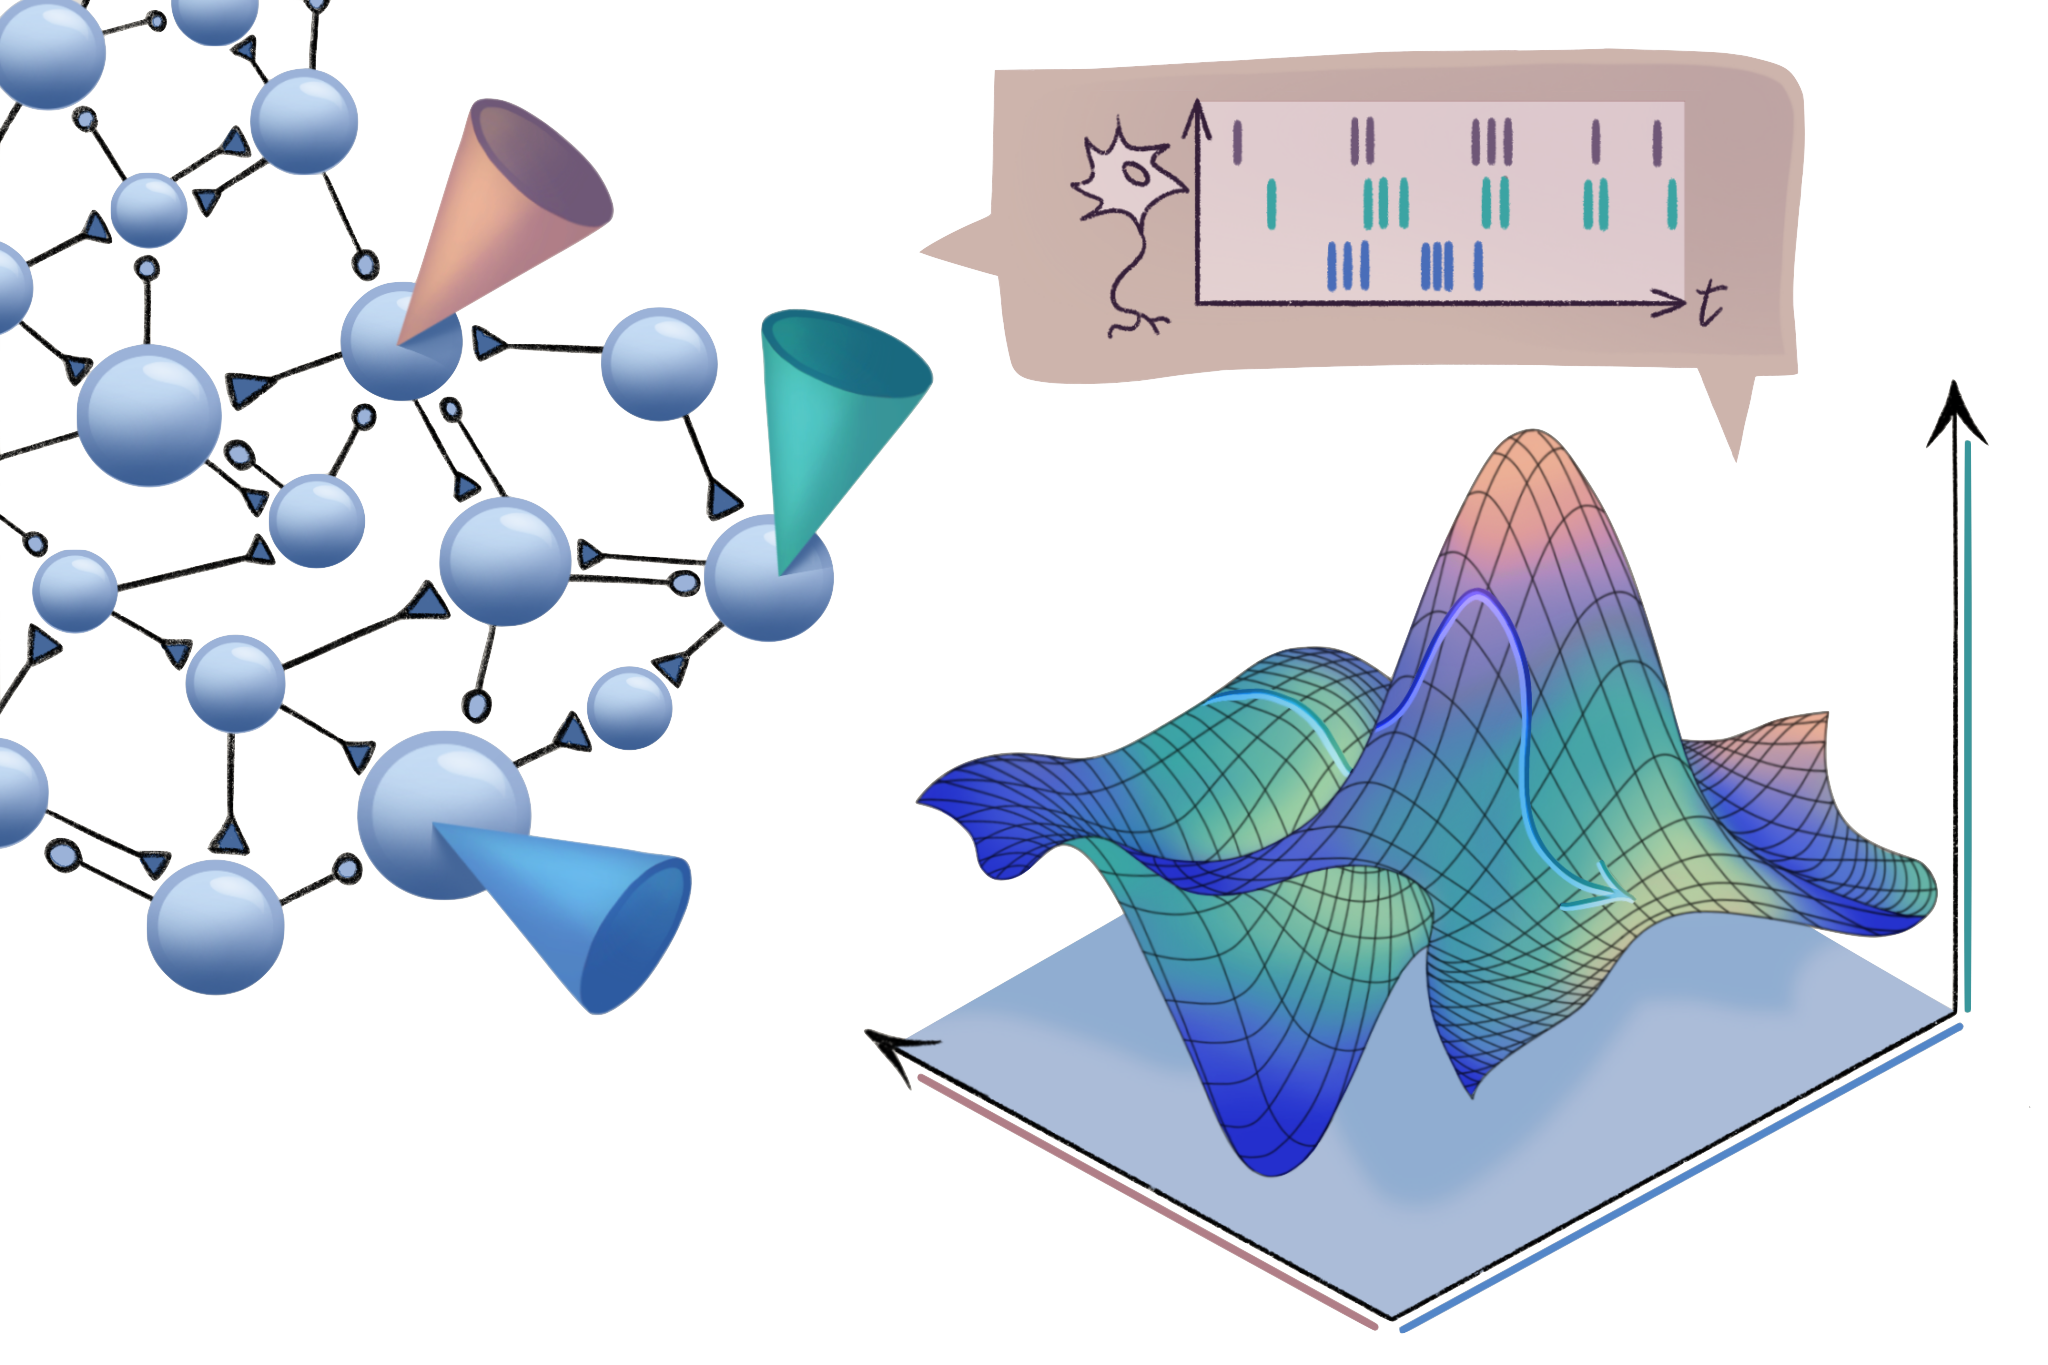
\includegraphics[width=\textwidth]{figs/manifold_schematic.png}
            \cite{Perich2024}
        \end{center}
    \end{columns}
\end{frame}

\begin{frame}{}
\textbf{Neural population geometry} refers to the configurations of these \textbf{neural manifolds} embedded in ambient \textbf{neural state space}~\cite{chung2021neural}
\end{frame}

\begin{frame}{Neural manifold formalism}
    \begin{itemize}
       \item $m$-dimensional manifold $\mathcal{M}$ is a topological space where each point $p \in \mathcal{M}$ has a neighborhood $U$ that is homeomorphic to an open subset of $\mathbb{R}^m$
       \item Let $\mathbf{r} = (r_1, r_2, \ldots, r_n) \in \mathbb{R}^n$ represent the firing rates of $n$ neurons at a given time. The neural manifold hypothesis posits that, during specific task execution, these population activity patterns do not explore the entire $n$-dimensional space but instead are constrained to a lower-dimensional subspace or manifold $\mathcal{M} \subset \mathbb{R}^n$, where typically $\dim(\mathcal{M}) \ll n$.
       \item E.g.,  
        $\mathcal{M}_{\text{obj}} = \{f(T_\theta(\mathbf{x})) : \theta \in \Theta\}$, $\mathbf{x} \in \mathbb{R}^d$ represents a stimulus and $T_\theta: \mathbb{R}^d \rightarrow \mathbb{R}^d$ represents a transformation with parameter $\theta$
    \end{itemize}
\end{frame}

\begin{frame}{Considerations for neural manifolds}
    \begin{itemize}
        \item \textbf{Neural variability}
        \begin{itemize}
       \item Neural responses vary due to stochastic processes in neural firing
       \item  Point clouds (clusters of points for each stimulus) define the empirical neural manifold
    \end{itemize}
        \item \textbf{Sparse sampling}
        \begin{itemize}
            \item Experimental limitations often allow only a finite sampling of possible stimuli or conditions leading to discrete approximation of continuous manifold
        \end{itemize} 
    \end{itemize}
\end{frame}

\begin{frame}{Neural manifold analysis methods}
    \begin{itemize}
        \item \textbf{Linear dimensionality reduction}: PCA
        
        \item \textbf{Nonlinear dimensionality reduction}: Isomap~\cite{tenenbaum2000global}, Locally Linear Embedding (LLE)~\cite{roweis2000nonlinear}, t-SNE~\cite{vandermaaten2008visualizing}, Multidimensional Scaling (MDS)~\cite{kruskal1964multidimensional}, PHATE~\cite{moon2019visualizing}, and UMAP~\cite{mcinnes2018umap}
        
        \item \textbf{Geometric approximation methods}: Convex hulls
        
        \item \textbf{Topologically-motivated methods}: Spline Parameterization for Unsupervised Decoding (SPUD)~\cite{chaudhuri2019intrinsic} 
        
        \item \textbf{Dynamics-based approaches}: Manifold Inference from Neural Dynamics (MIND)~\cite{low2018probing}
        
        
        \item \textbf{Density-based approaches}: Kernel Density Estimation (KDE)
    \end{itemize}
\end{frame}

\begin{frame}{Properties of interest}
    \begin{columns}
        \column{0.3\textwidth}
        \begin{itemize}
            \item Dimensionality
            \item Curvature
            \item Separability
            \item Capacity
        \end{itemize}
        \column{0.5\textwidth}
        \begin{center}
            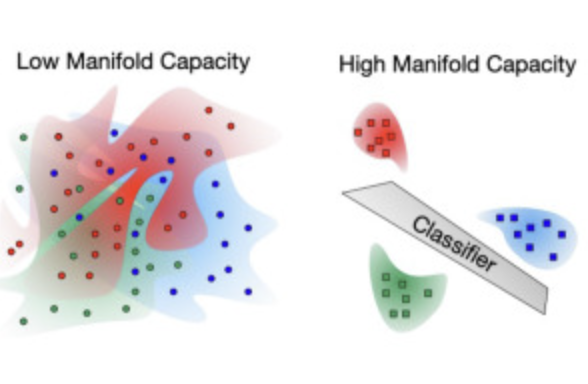
\includegraphics[width=\textwidth]{figs/capacity.png}
            \cite{chung2021neural}
        \end{center}
    \end{columns}
\end{frame}

\section{Neural geometry of an ANN}

\begin{frame}{Task input}
    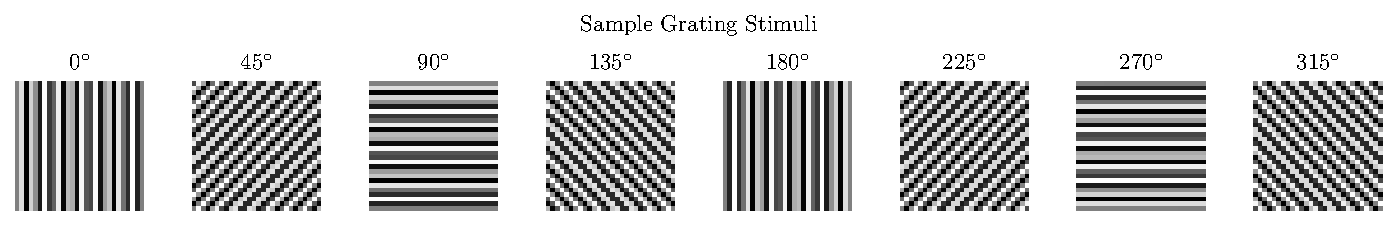
\includegraphics[width=\textwidth]{results/grating_samples.pdf}
\end{frame}

\begin{frame}{Architecture}
    \begin{center}
    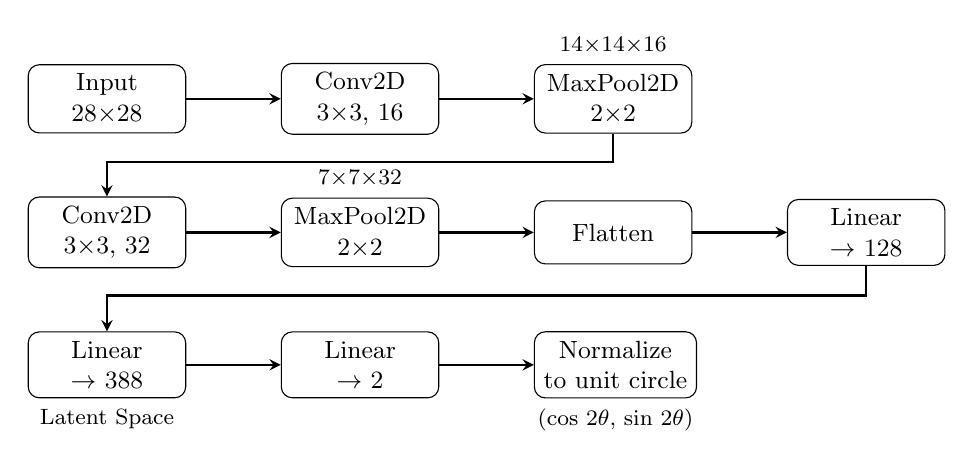
\begin{tikzpicture}[
        node distance=1.2cm,
        box/.style={
            rectangle,
            draw,
            minimum width=2cm,
            minimum height=0.8cm,
            align=center,
            rounded corners,
            font=\small
        },
        arrow/.style={
            ->,
            thick,
            >=stealth
        }
    ]

    % Input layer
    \node[box] (input) {Input\\28$\times$28};

    % First conv block
    \node[box, right=of input] (conv1) {Conv2D\\3$\times$3, 16};
    \node[box, right=of conv1] (pool1) {MaxPool2D\\2$\times$2};

    % Second conv block
    \node[box, below=0.8cm of input] (conv2) {Conv2D\\3$\times$3, 32};
    \node[box, right=of conv2] (pool2) {MaxPool2D\\2$\times$2};

    % Flatten and FC layers
    \node[box, right=of pool2] (flatten) {Flatten};
    \node[box, right=of flatten] (fc1) {Linear\\$\rightarrow$ 128};
    
    % Second row of FC layers
    \node[box, below=0.8cm of conv2] (fc2) {Linear\\$\rightarrow$ 388};
    \node[box, right=of fc2] (output_raw) {Linear\\$\rightarrow$ 2};
    \node[box, right=of output_raw] (output_norm) {Normalize\\to unit circle};

    % Connections - modified to create column-like flow
    \draw[arrow] (input) -- (conv1);
    \draw[arrow] (conv1) -- (pool1);
    
    % Modified connections to go down and then across instead of diagonal
    \draw[arrow] (pool1) -- ++(0,-0.8cm) -| (conv2);
    \draw[arrow] (conv2) -- (pool2);
    \draw[arrow] (pool2) -- (flatten);
    \draw[arrow] (flatten) -- (fc1);
    
    % Modified connection to go down and then across
    \draw[arrow] (fc1) -- ++(0,-0.8cm) -| (fc2);
    \draw[arrow] (fc2) -- (output_raw);
    \draw[arrow] (output_raw) -- (output_norm);

    % Add dimensions as labels
    \node[above=0.01cm of pool1, font=\footnotesize] {14$\times$14$\times$16};
    \node[above=0.01cm of pool2, font=\footnotesize] {7$\times$7$\times$32};
    \node[below=0.01cm of fc2, font=\footnotesize] {Latent Space };
    \node[below=0.01cm of output_norm, font=\footnotesize] {(cos 2$\theta$, sin $2\theta$)};

    \end{tikzpicture}
\end{center}
\end{frame}

\begin{frame}{Analysis of latent space activity}
    \[
\underbrace{
\begin{bmatrix}
    \circ & \circ & \cdots & \circ \\
    \circ & \circ & \cdots & \circ \\
    \vdots & \vdots & \ddots & \vdots \\
    \circ & \circ & \cdots & \circ
\end{bmatrix}}_{388 \times 18}
\quad
\overset{\text{PCA}}{\longrightarrow}
\quad
\underbrace{
\begin{bmatrix}
    \circ & \circ & \cdots & \circ \\
    \circ & \circ & \cdots & \circ
\end{bmatrix}}_{2 \times 18}
\]
\end{frame}

\begin{frame}{PCA projection reveals directional circular structure}
    \begin{center}
        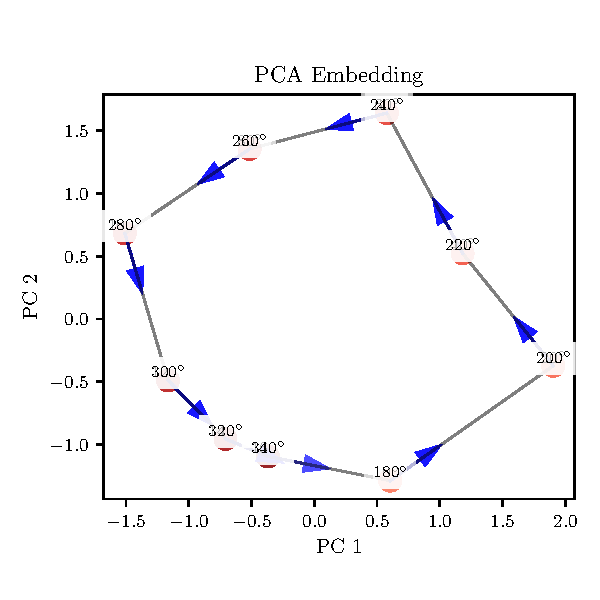
\includegraphics[width=0.6\textwidth,trim={0 1cm 0 1cm},clip]{results/ann_circular_colormap_visualization.pdf} 
    \end{center}
\end{frame}

\section{Neural geometry of a biological neural circuit}

\section{Conclusions}

\section{References}
\begin{frame}[allowframebreaks]{References}
    \bibliographystyle{apalike}
\bibliography{refs}
\end{frame}
\end{document} 